%%%%%%%%%%%%
%
% $Autor: Wings $
% $Datum: 2019-03-05 08:03:15Z $
% $Pfad: Automatisierung/Skript/Produktspezifikation/Powerpoint/AMF.tex $
% $Version: 4250 $
% !TeX spellcheck = en_GB/de_DE
% !TeX encoding = utf8
% !TeX root = filename 
% !TeX TXS-program:bibliography = txs:///biber
%
%%%%%%%%%%%%


\chapter{Gesichtserkennung mit Edge Impulse}

In diesem Kapitel wird eine Modell zur Gesichtserkennung mit Hilfe der Plattform Edge IMpulse\Mynote{Quelle}\index{Edge IMpulse} entwickelt. Ein weiteres Werkzeug, beispielsweise OpenMV IDE, wird nicht benötigt. Das Flussdiagramm für den Gesamtprozess ist in der folgenden Abbildung \ref{FaceFlowChart} dargestellt. 

\begin{figure}[H]
	\centering
	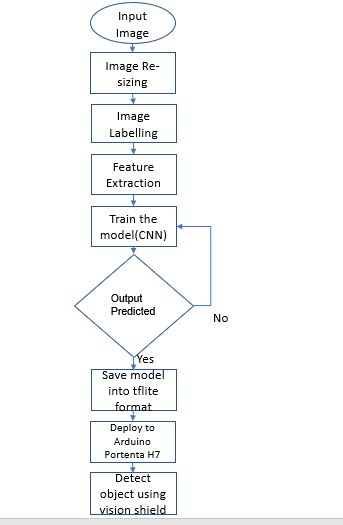
\includegraphics[width=\textwidth]{Arduino/flowchart2}
	\caption{Flussdiagramm des Gesamtprozesses}
	\label{FaceFlowChart}
\end{figure}


\section{Datenbank}  

Zum Training der Modells wird der Datensatz UTKFace, siehe Kapitel \ref{UTKFace}, verwendet. Es können aber auch eigene Bilder hinzugefügt werden. Letztlich setzt sich der verwendete Datensatz wie folgt zusammen:

\begin{itemize}
	\item Manuell aufgenommene Bilder von der Kamera, Bilder aus dem UTKFace-Datensatz.
	\item Trainingssatz: Bestehend aus 388 Bildern
	\item Testsatz: bestehend aus 98 Bildern
\end{itemize}

\bigskip



Da unser Datensatz nun vorbereitet ist, können wir das Modell auf dem Plattforom Edge Impulse\index{Edge Impulse} trainieren. Zu diesem Zweck müssen wir ein Projekt auf der Edge Impulse-Plattform erstellen. Dies ist in Kapitel \ref{EdgeImpulseNewProject} beschrieben. Um Bilder, die sich auf dem Arduino Board befinden, hochzuladen, muss der Arduino zuerst mit der Plattform Edge Impulse verbunden werden. Dies wird im Abschnitt \ref{EdgeImpulseArduinoConnect} beschrieben.






	\subsection{Kennzeichnung von Daten}
	
	Nachdem unsere Daten hochgeladen wurden, müssen wir sie nun beschriften. Dazu gehen wir auf die Option \glqq Labelling Queue\grqq{} in der Datenerfassung und beginnen mit dem Zeichnen eines Begrenzungsrahmens um das Objekt und beschriften es. In unserer Datenbank haben wir zwei verschiedene Objekte, nämlich Flächen und Stifte. Wir zeichnen also manuell einen Begrenzungsrahmen um das Objekt und beschriften ihn für alle Bilder im Datensatz. \ref{ImageLabelling}
	
	\begin{figure}[H]
		\centering
		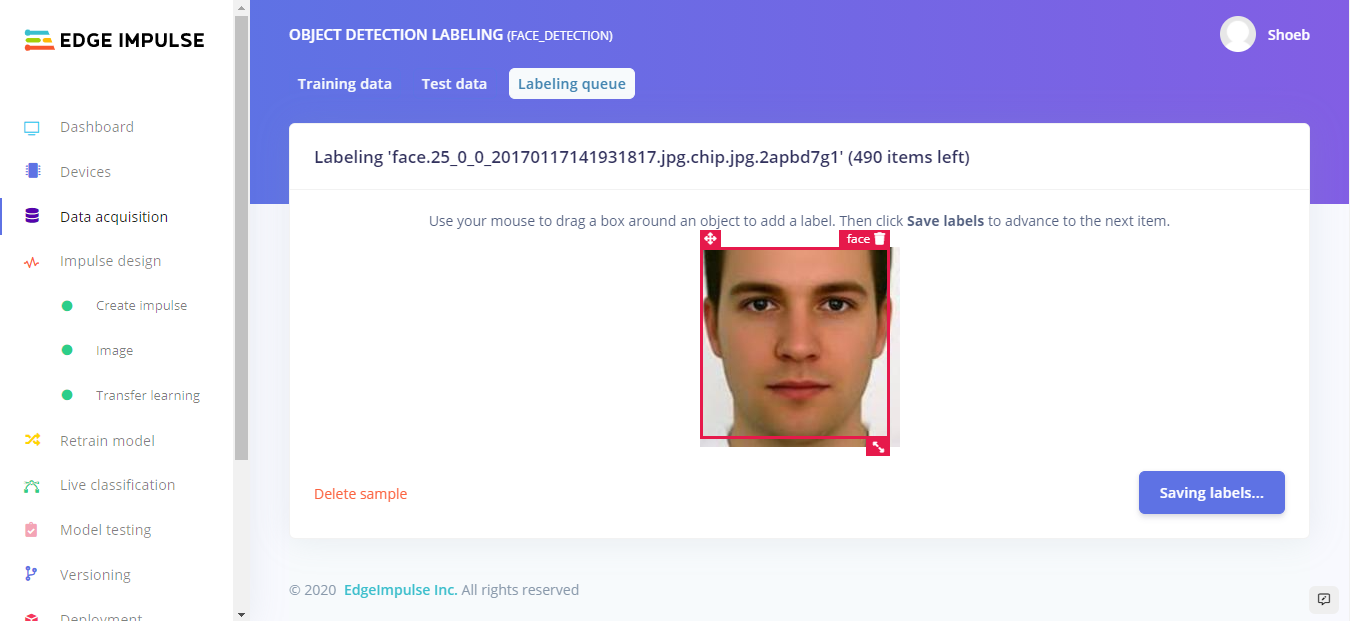
\includegraphics[width=\textwidth]{Arduino/labelface}
		\caption{Beschriftung eines Bildes }
		\label{ImageLabelling}
	\end{figure}
	
	
	\section{Umwandlung von Daten}
	
	\subsection{Die Gestaltung des Impulses}
	
	\textbf{Vorverarbeitung von Bildern:}
	
	Um den Impuls zu entwerfen, klicken Sie auf Impulsdesign und stellen Sie dann die Bildbreite und -höhe auf $320\times 320$ ein, da das vortrainierte Objekterkennungsmodell nur mit Bildern dieser Größe funktioniert \cite{EdgeImpulse:2021}. Der Bildvorverarbeitungsblock nimmt das Eingabebild auf und kann es optional in Graustufen umwandeln und die Daten dann in ein Merkmalsfeld umwandeln.  Dann klicken wir auf den Lernblock und wählen Objekterkennung. Klicken Sie dann auf Impuls speichern, wie in der Abbildung \ref{EdgeImpulseCreate} gezeigt.
	
	\begin{figure}[H]
		\centering
		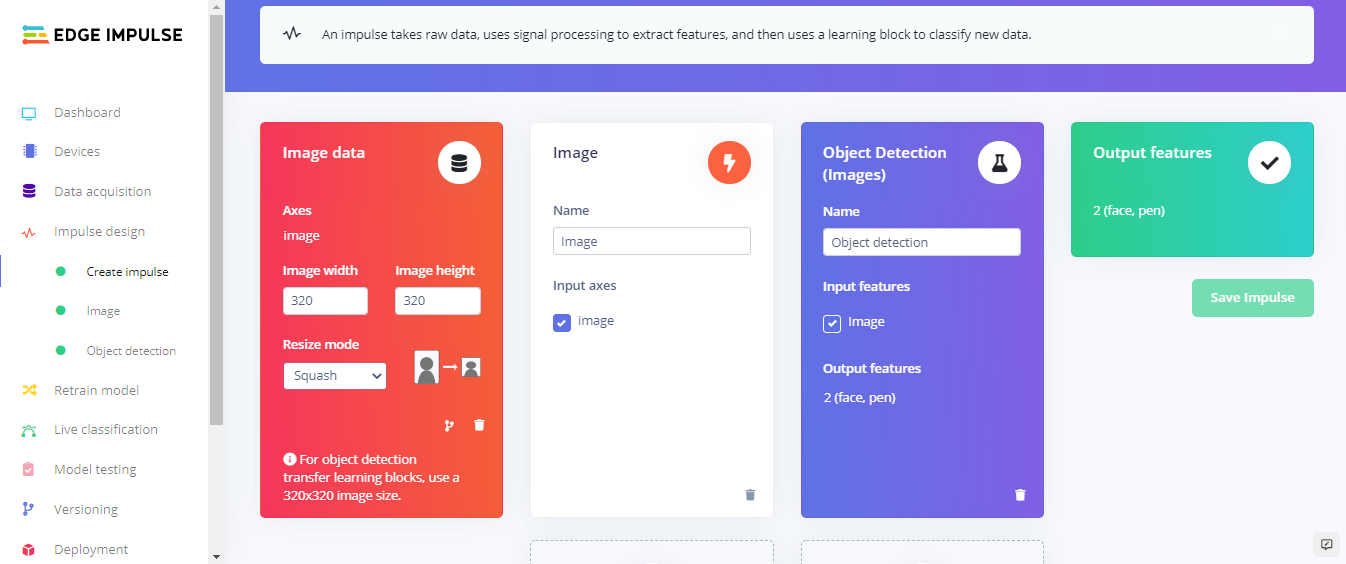
\includegraphics[width=\textwidth]{Arduino/createimpulse}
		\caption{Impulse schaffen}
		\label{EdgeImpulseCreate}
	\end{figure}
	
	\subsection{Konfigurieren des Bildverarbeitungsblocks} 
	
	Um den Verarbeitungsblock zu konfigurieren, klicken Sie im Menü auf der linken Seite auf Bilder. Dies zeigt uns die Rohdaten oben auf dem Bildschirm und die Ergebnisse des Verarbeitungsschritts rechts. Wir können auch die Optionen verwenden, um zwischen den Modi \glqq RGB\grqq{} und \glqq Grayscale\grqq{} zu wechseln. Klicken Sie dann auf Parameter speichern, wie in Abbildung \ref{EdgeImpulseSave} gezeigt. 
	
	\begin{figure}[H]
		\centering
		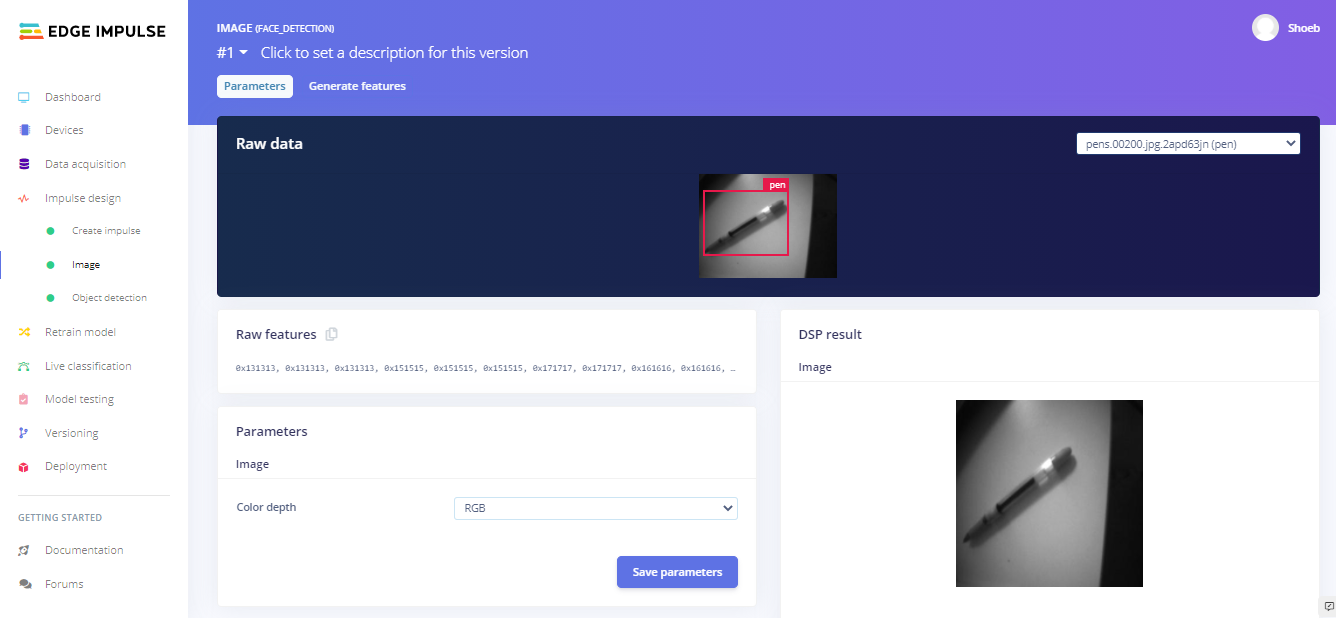
\includegraphics[width=\textwidth]{Arduino/saveparameters}
		\caption{Parameter speichern}
		\label{EdgeImpulseSave}
	\end{figure}
	
	Klicken Sie dann oben auf die Option \glqq generate features\grqq{} und dann auf \glqq generate features\grqq{}. In der Abbildung \ref{EdgeImpulseGenerateFeature} ist zu sehen, dass die aus dem Datensatz der Bilder, die aus Stiften und Gesichtern bestehen, generierten Merkmale leicht zu erkennen sind.
	
	\begin{figure}[H]
		\centering
		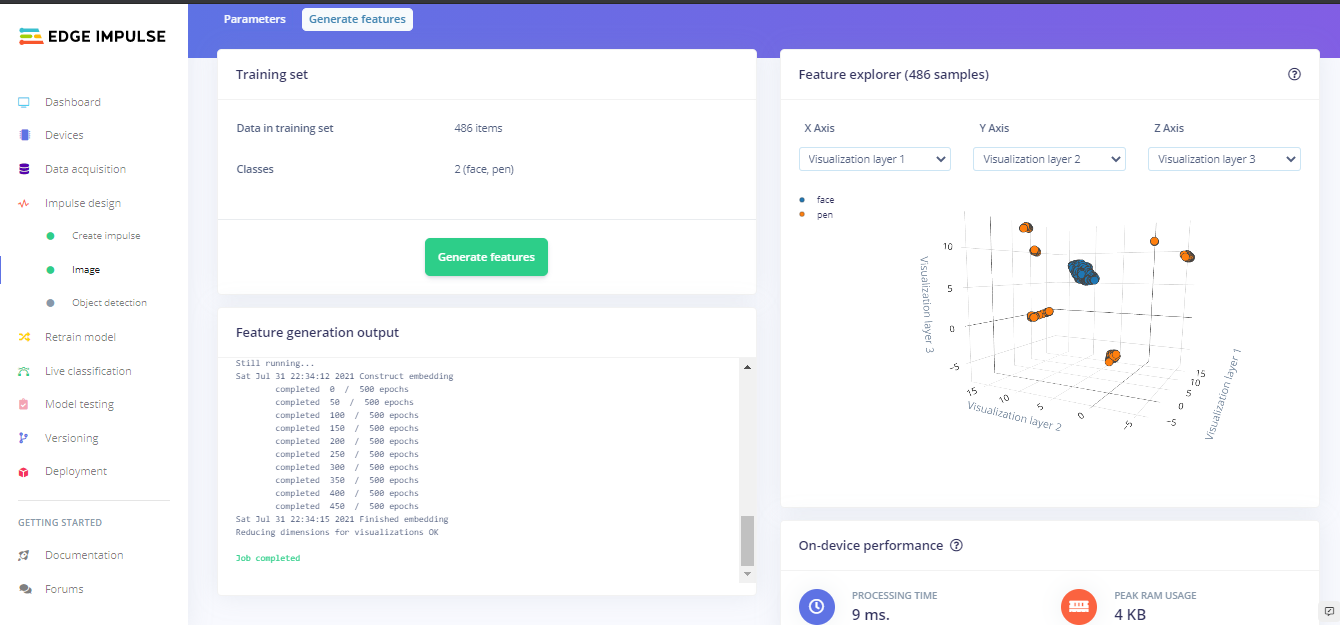
\includegraphics[width=\textwidth]{Arduino/featuregenerate}
		\caption{Merkmale generieren}
		\label{EdgeImpulseGenerateFeature}
	\end{figure}
	
	\section{Data training}
	
	\textbf{Konfigurieren des Transfer-Learning-Modells:}
	
	In diesem Fall verwenden wir den Transfer-Learning-Block, da es einfacher ist, ein bereits trainiertes Modell zu verwenden, indem nur die oberen Schichten eines neuronalen Netzes beibehalten werden, und wir das Modell dann in kurzer Zeit trainieren können. Um das Transfer-Learning-Modell zu konfigurieren, klicken Sie auf Objekterkennung. Hier können wir die Lernrate einstellen, in unserem Fall haben wir sie auf 0,15 und die Anzahl der Trainingszyklen auf 25 eingestellt. Dann wählen wir das Basismodell aus, in unserem Fall MobileNetV2\index{MobileNetV2}, und klicken dann auf Training starten.  Nachdem der Trainingsprozess abgeschlossen ist, können wir in der Abbildung \ref{EdgeImpulseCompletedTraining} sehen, dass die Genauigkeit 87\% beträgt.
	
	\begin{figure}[H]
		\centering
		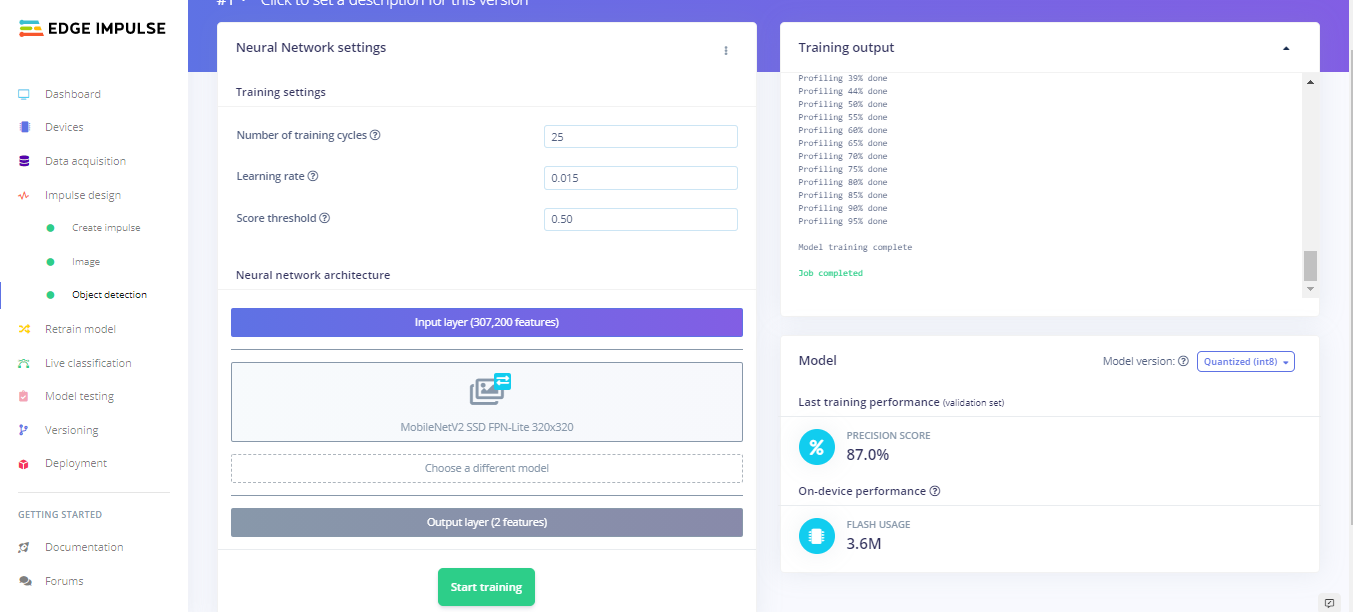
\includegraphics[width=\textwidth]{Arduino/Trainedmodel}
		\caption{Abgeschlossenes Training}
		\label{EdgeImpulseCompletedTraining}
	\end{figure}
	
	\section{Prüfung des Modells}
	
	Um das Modell zu testen, müssen wir auf die Option \glqq model testing\grqq{} und dann auf \glqq classify all\grqq{} klicken. Hier wurden die Bilder des Datensatzes automatisch in Trainings- und Testbilder unterteilt. In diesem Fall hat das Modell die Eingabebilder in Trainingsbilder mit 388 Bildern und Testbilder mit 98 Bildern unterteilt. Die Testbilder werden dann verwendet, um zu überprüfen, wie gut das Modell funktioniert. Wie aus der Abbildung \ref{EdgeImpulseTestingModel} hervorgeht, erreichte das Modell eine Genauigkeit von 87,1 \%.
	
	\begin{figure}[H]
		\centering
		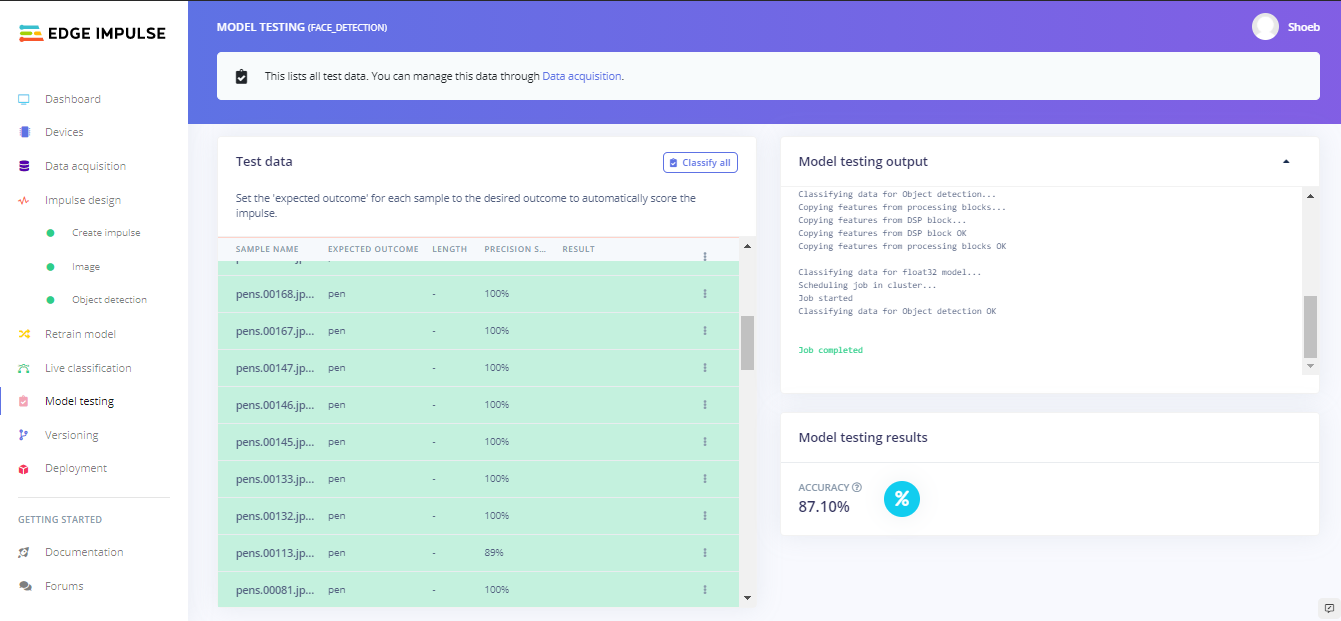
\includegraphics[width=\textwidth]{Arduino/testmodel}
		\caption{Prüfung des Modells}
		\label{EdgeImpulseTestingModel}
	\end{figure}
	
	Wir können auch die Live-Klassifizierung durchführen und Objekte in Echtzeit mit dem Vision Shield erkennen.  Klicken Sie im Menü auf die Option \glqq live classification\grqq{}  und verbinden Sie unser Portenta H7-Gerät mit dem Edge Impulse, indem Sie das Gerät auswählen. Sobald es angeschlossen ist, können wir den Kamerastream vom Vision Shield sehen. Hier haben wir das Modell getestet, indem wir uns auf das Gesicht konzentriert haben, und wie wir in der Abbildung \ref{EdgeImpulseLiveClassification} sehen können, gibt es die Ausgabe als Gesicht mit einem Wert von 0,89, was eine ziemlich gute Vorhersage ist.
	
	\begin{figure}[H]
		\centering
		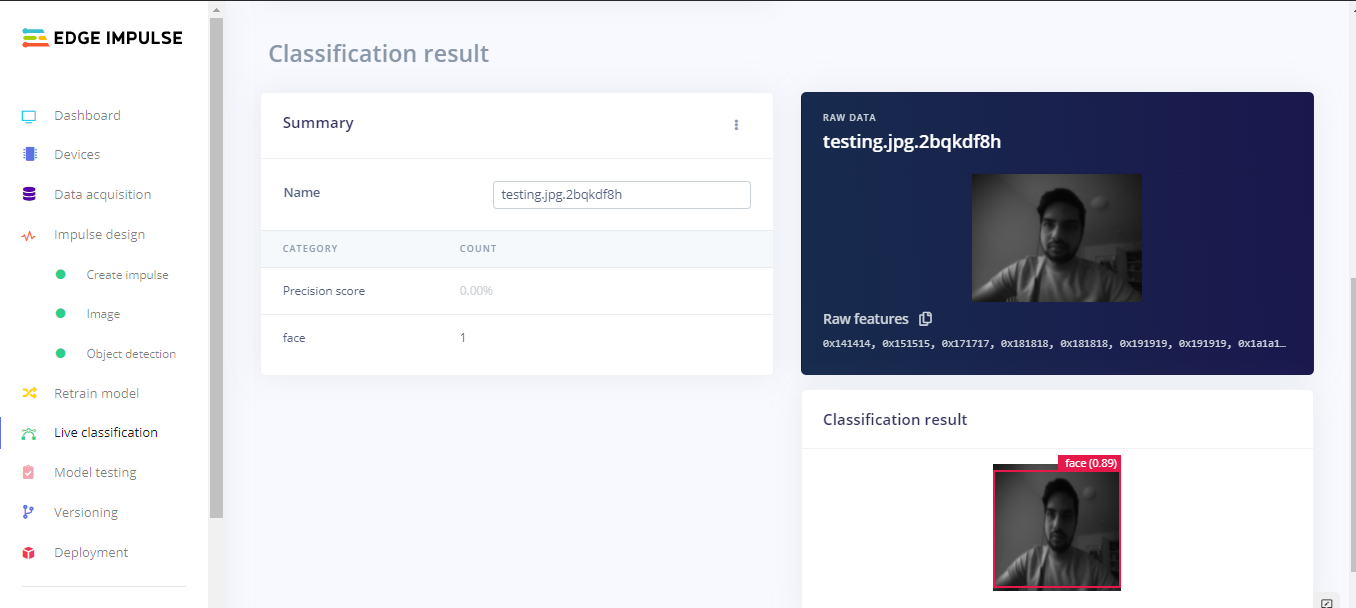
\includegraphics[width=\textwidth]{Arduino/liveclassification}
		\caption{Live-Klassifizierung mit Hilfe der Vision-Shield-Kamera}
		\label{EdgeImpulseLiveClassification}
	\end{figure}
	
\Mynote{Im Programm wird die Methode tf.classify	verwendet. Details!!!}
